\documentclass[12pt,a4paper]{report}

\usepackage[francais]{babel}
\usepackage[utf8]{inputenc}
\usepackage{epigraph}
\usepackage[T1]{fontenc}
\usepackage{listings}
\usepackage{graphicx}
\usepackage{parskip}
\usepackage{xcolor}
\usepackage{hyperref}
\usepackage{titlesec}


%% config
\definecolor{deepblue}{rgb}{0,0,0.5}

\titleformat{\chapter}[display]
  {\normalfont\bfseries}{}{0pt}{\Large}

\lstset{
  literate=
  {á}{{\'a}}1 {é}{{\'e}}1 {í}{{\'i}}1 {ó}{{\'o}}1 {ú}{{\'u}}1
  {Á}{{\'A}}1 {É}{{\'E}}1 {Í}{{\'I}}1 {Ó}{{\'O}}1 {Ú}{{\'U}}1
  {à}{{\`a}}1 {è}{{\`e}}1 {ì}{{\`i}}1 {ò}{{\`o}}1 {ù}{{\`u}}1
  {À}{{\`A}}1 {È}{{\'E}}1 {Ì}{{\`I}}1 {Ò}{{\`O}}1 {Ù}{{\`U}}1
  {ä}{{\"a}}1 {ë}{{\"e}}1 {ï}{{\"i}}1 {ö}{{\"o}}1 {ü}{{\"u}}1
  {Ä}{{\"A}}1 {Ë}{{\"E}}1 {Ï}{{\"I}}1 {Ö}{{\"O}}1 {Ü}{{\"U}}1
  {â}{{\^a}}1 {ê}{{\^e}}1 {î}{{\^i}}1 {ô}{{\^o}}1 {û}{{\^u}}1
  {Â}{{\^A}}1 {Ê}{{\^E}}1 {Î}{{\^I}}1 {Ô}{{\^O}}1 {Û}{{\^U}}1
  {œ}{{\oe}}1 {Œ}{{\OE}}1 {æ}{{\ae}}1 {Æ}{{\AE}}1 {ß}{{\ss}}1
  {ű}{{\H{u}}}1 {Ű}{{\H{U}}}1 {ő}{{\H{o}}}1 {Ő}{{\H{O}}}1
  {ç}{{\c c}}1 {Ç}{{\c C}}1 {ø}{{\o}}1 {å}{{\r a}}1 {Å}{{\r A}}1
  {€}{{\EUR}}1 {£}{{\pounds}}1,
    language={Python},
    basicstyle=\ttfamily\small, 
    tabsize=4,
    keywordstyle=\bold,
    commentstyle=\color{gray},
    backgroundcolor=\color{lightgray},
    otherkeywords={self},
    keywordstyle=\ttfamily\small\color{deepblue},
    frame=single
    showtabs=false,
    showspaces=false,
    showstringspaces=false
}

\renewcommand{\labelitemi}{∙}
%%macro

\renewcommand{\path}[1]{\texttt{#1}}

\newcommand{\codeintext}[1]{\texttt{#1}}

\begin{document}


\title{{\huge Introduction à Godot}\\
\vspace{3cm}

\includegraphics[width=8cm]{img/godot_logo.jpg}
}
\author{Bastien Gorissen \& Thomas Stassin}
\date{Année 2016}

\maketitle
\tableofcontents

\chapter*{Introduction}
\addcontentsline{toc}{chapter}{Introduction}

Le but de ce cours est de vous faire découvrir Godot\footnote{\url{http://www.godotengine.org/}}, un moteur de jeu libre et open source. Ce moteur est capable de produire des jeux 2D ainsi que 3D, bien que le cours se concentrera sur la partie 2D des outils proposés.

Tout au long de ce cours, nous aurons l'occasion d'élaborer un projet modeste, avec quelques sous-projets en cours de route afin de voir les fonctionnalités dans un cadre isolé.

\chapter{Level 1 : Mon premier jeu en Godot}

Pour ce premier contact avec Godot, nous allons tenter de réaliser un petit jeu sans prétention. Il s'agira d'un jeu où il faut attraper certains objets qui tombent du haut de l'écran, tout en évitant certains autres.

\section{Création du projet}

Quand vous lancez Godot, vous serez saluées par un écran comme celui de la figure \ref{lvl1-screen1}. Au premier lancement, il sera vide, mais vous verrez que bientôt il se remplira de tous les projets que vous aurez créés.

\begin{figure}
  \begin{center}
    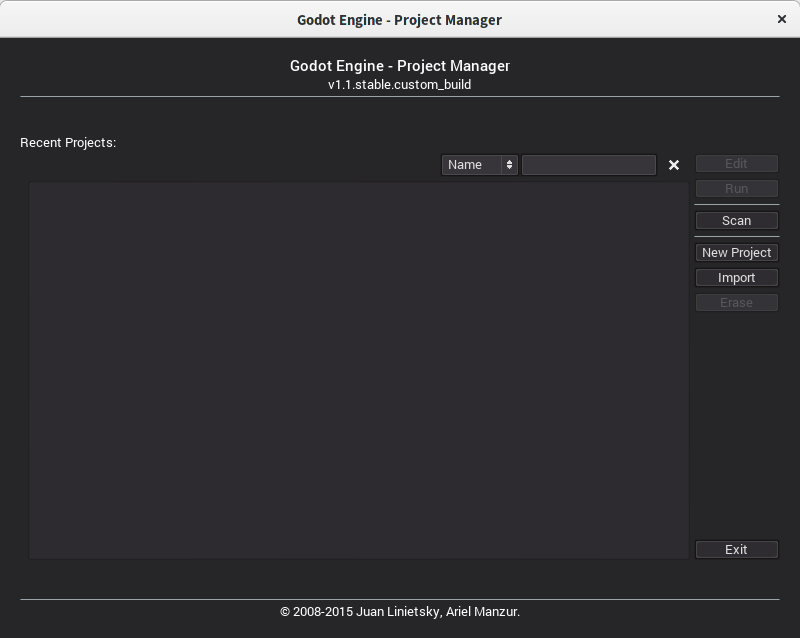
\includegraphics[width=12cm]{img/lvl1-screen1.png}
  \end{center}
  \caption{\label{lvl1-screen1} L'écran de sélection de projets de Godot, sa façon de vous dire bonjour.}
\end{figure}

Le bouton qui nous intéresse plus particulièrement est le bouton \emph{New Project}, qui va nous permettre de... créer un nouveau projet (qui l'eut crû). Vous verrez une popup s'ouvrir, comme sur la figure \ref{lvl1-screen2}.

\begin{figure}
  \begin{center}
    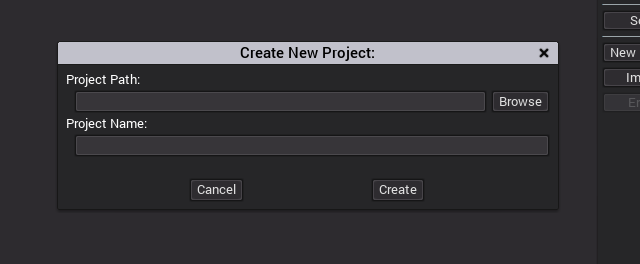
\includegraphics[width=10cm]{img/lvl1-screen2.png}
  \end{center}
  \caption{\label{lvl1-screen2} Un nouveau projet ! Sentez-vous l'excitation qui monte, la hype qui se profile ? Non ? Ah bon...}
\end{figure}

En utilisant le bouton \emph{Browse}, vous pourrez naviguer jusqu'à trouver un endroit parfait pour votre projet. Tous les fichiers du projet seront stockés dans ce dossier. En plus, Godot vous encourage à donner un nom intelligent à votre dossier: par défaut, le nom du dossier sera également le nom du projet. Dans un énorme élan de créativité, j'ai décidé d'appeler mon dossier \codeintext{FallingThings}, d'après le principe de notre jeu.

Une fois la boite de dialogue remplie et validée, vous aurez l'insigne honneur de voir votre nouveau projet apparaître dans la fenêtre de sélection de projets (voir figure \ref{lvl1-screen3}).

\begin{figure}
  \begin{center}
    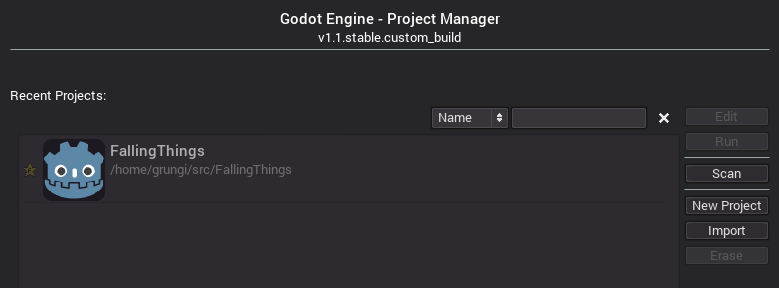
\includegraphics[width=12cm]{img/lvl1-screen3.png}
  \end{center}
  \caption{\label{lvl1-screen3} Et voilà, le projet est maintenant prêt à être ouvert, et le travail va pouvoir commencer.}
\end{figure}

Les choses sérieuses peuvent commencer !

\section{Le Nouveau Monde}

Tels des exploratrices devant les côtes d'une île inconnue, vous avez ouvert votre projet, et vous vous êtes retrouvées devant un écran relativement intimidant. Pas très loin de celui de la figure \ref{lvl1-screen4}.

\begin{figure}
  \begin{center}
    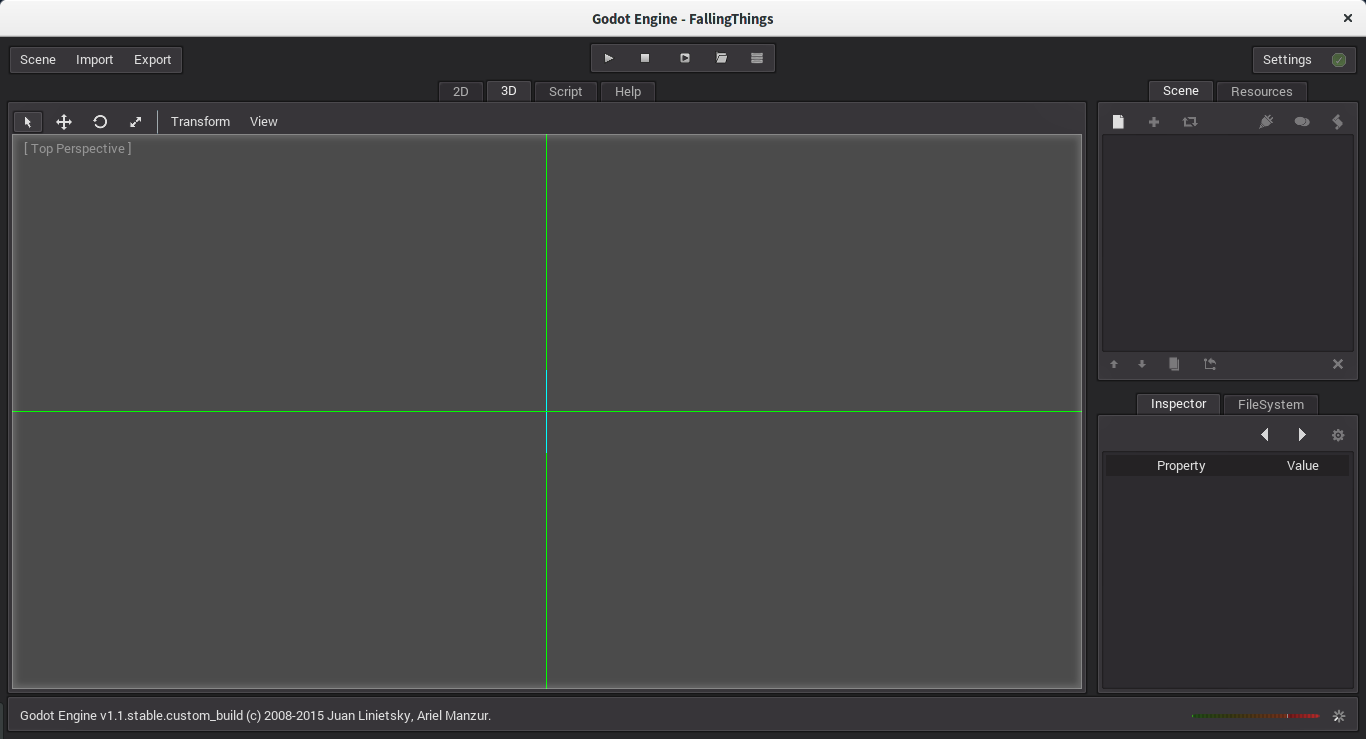
\includegraphics[width=12cm]{img/lvl1-screen4.png}
  \end{center}
  \caption{\label{lvl1-screen4} Des icones, des boutons, des onglets... Bienvenue dans Godot !}
\end{figure}

Pas de panique cependant, c'est plus simple qu'il n'y parait. L'écran est divisé 5 zones principales.

\begin{description}
\item[En haut] : On retrouve des menus, que nous explorerons petit à petit, une barre de boutons qui permettent de lancer le jeu, le stopper, lancer une \emph{scène}, et un bouton sur la droite permettant de modifier certains paramètres de l'éditeur de Godot.
\item[Au centre] : La majeure partie de l'écran est occupée par la zone de travail principal de Godot. Comme un navigateur, elle se présente sous la forme de plusieurs onglets. Le premier de ceux-ci offre une vue 2D de l'application (nous allons souvent l'utiliser), le deuxième sert dans le cadre de projets 3D, le troisième sert à éditer les scripts (le code), et le dernier vous offre l'aide de Godot, bien utile à avoir sous la main.
\item[A droite, en haut] : Vous trouverez là la hiérarchie des \emph{noeuds} présents dans la \emph{scène} en cours. Ce charabia deviendra plus intelligible quand nous parlerons de comment Godot organise les éléments des projets un peu plus loin. Mais retenez que c'est là que vous trouverez les différents éléments qui sont actuellement dans votre jeu. Le second onglet, \emph{Resources}, vous montrera les différentes sources de données (textures, sprites, fichiers sons, ...) qui seront utilisées dans le projet. Nous y reviendrons également plus tard.
\item[A droite, en bas] : Là où l'onglet \emph{Scene} ci-dessus vous montrait la liste des éléments de la \emph{scène}, l'onglet \emph{Inspector} vous renseigne les propriétés de l'objet actuellement sélectionné. Vous pourrez l'utiliser pour définir un grand nombre d'options pour chaque objet. A ses côtés, l'onglet \emph{FileSystem} vous montre simplement un navigateur qui vous permet de parcourir l'arborescence des dossiers de votre projet.
\item[En bas] : Tout en bas de la fenêtre, vous trouverez une barre de statut, qui vous montrera les sorties générées par les commandes que vous utiliserez ou par votre jeu. En cliquant dessus, vous pourrez faire apparaître une zone plus conséquente où vous pourrez voir plus de texte.
\end{description}

Voilà, maintenant que vous êtes familiarisées avec l'organisation générale de l'interface du moteur, il est temps de voir comment utiliser tout cela.

\section{Le \emph{noeud} du problème}

Nous allons maintenant aborder une notion vraiment centrale à l'organisation de Godot: les \emph{noeuds}, ou \emph{nodes} en Anglais.

Le concept va être abstrait pendant quelques lignes, mais nous verrons tout de suite comment l'utiliser en pratique.

Le \emph{noeud} est, dans Godot, l'élément de base avec lequel vous allez créer vos jeux. Depuis un sprite pour représenter un personnage à une source de lumière pour l'éclairer, en passant par une zone déterminant la fin d'un niveau, tout dans Godot est un \emph{noeud}. Plus que ça, les \emph{noeuds} sont définis comme ayant les caractéristiques suivantes:

\begin{enumerate}
\item Un \emph{noeud} a un nom.
\item Un \emph{noeud} possède un ensemble de \emph{propriétés} éditables.
\item Un \emph{noeud} peut faire appel à du code pour remplir son rôle.
\item Un \emph{noeud} peut être ajouté à un autre \emph{noeud} en tant qu'enfant.  
\end{enumerate}

Si les trois premières propriétés sont importantes, c'est la quatrième qui mérite que l'on s'y attarde. En effet, le fait de pouvoir organiser les \emph{noeuds} de façon hiérarchique permet de concevoir des constructions complexes, tout en conservant chaque \emph{noeud} isolé et simple.

Par exemple, on pourrait imaginer un \emph{noeud} pour afficher un personnage 2D, qui aurait pour enfant un \emph{noeud} pour gérer son animation, un autre pour jouer les effets sonores qui lui sont propres, etc. Nous aurons l'occasion de faire usage de cette façon de faire rapidement, vous verrez, c'est très utile ! Mais pour le moment, il suffit de retenir que les \emph{noeuds} peuvent être organisés comme sur la figure \ref{lvl1-nodetree}.

\begin{figure}
  \begin{center}
    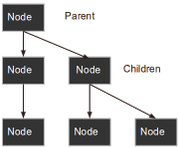
\includegraphics[width=6cm]{img/lvl1-nodetree.png}
  \end{center}
  \caption{\label{lvl1-nodetree} Exemple de hiérarchie de \emph{noeuds}.}
\end{figure}

Mais assez de théorie, passons à l'action !

\section{Première visite au magasin de jouets}

Il est temps de créer nos premiers \emph{noeuds}, et d'enfin voir quelque chose dans notre projet vide. En haut à droite de votre écran, dans l'onglet \emph{Scene}, vous trouverez une petite icône de page blanche, comme sur la figure \ref{lvl1-screen5}. Si vous passez le curseur de votre souris dessus, une info-bulle vous apprendra qu'il s'agit d'un bouton prévu pour créer un nouveau \emph{noeud}, ajoutant en plus un raccourci bien pratique pour faire la même chose : \codeintext{Ctrl + A}.


\begin{figure}
  \begin{center}
    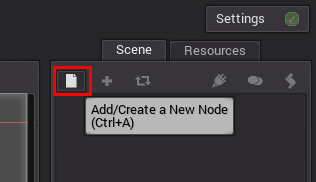
\includegraphics[width=6cm]{img/lvl1-screen5.png}
  \end{center}
  \caption{\label{lvl1-screen5} Le bouton magique.}
\end{figure}

Si vous cliquez sur ledit bouton (ou utilisez le raccourci clavier, selon), une nouvelle fenêtre va s'ouvrir, avec tout un tas de choses dedans. Voyez plutôt à la figure \ref{lvl1-screen6}.

\begin{figure}
  \begin{center}
    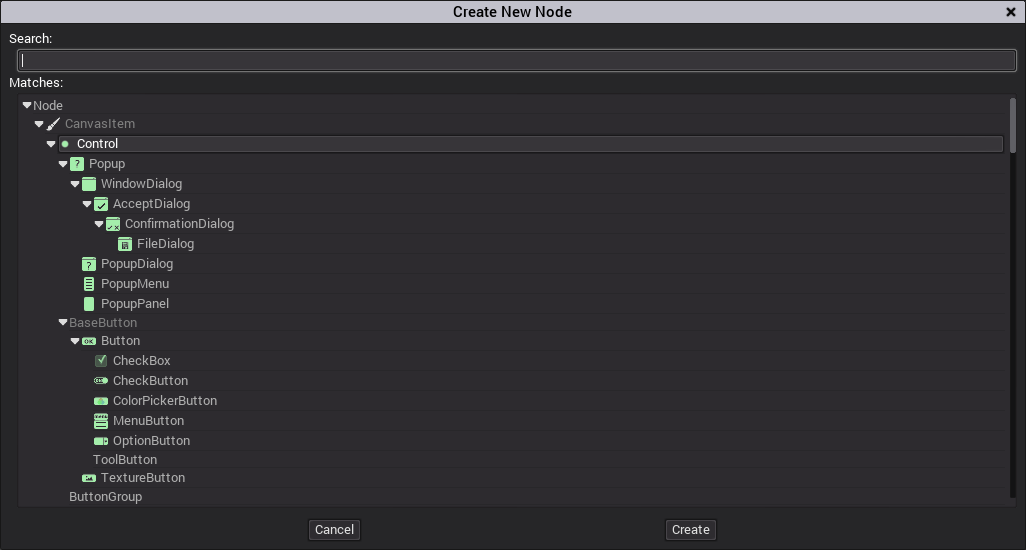
\includegraphics[width=8cm]{img/lvl1-screen6.png}
  \end{center}
  \caption{\label{lvl1-screen6} Votre magasin de jouets perso !}
\end{figure}

Comme dans un vrai magasin, des objets de toutes les couleurs sont en compétition pour votre attention, et sont organisés d'une manière qui, si elle n'est pas apparente de prime abord, l'est à l'usage. La première chose que vous pourrez remarquer est que les différents objets sont principalement regroupés par couleur. Pour vous y retrouver, voici les trois couleurs principales :

\begin{description}
\item[Vert] pour tout ce qui touche aux interfaces utilisateur (boutons, boites de dialogue, ...)
\item[Bleu] pour tout ce qui est 2D. C'est la couleur qui nous sera la plus utile !
\item[Rouge] pour tout ce qui est 3D. Comme expliqué dans le préambule de ce cours, nous n'aurons pas vraiment l'occasion de nous pencher sur le sujet, mais il est bon de savoir ce qui existe dans Godot.
\end{description}

Les autres couleurs sont plus mineures, et moins essentielles (ou ne sont pas dans une catégorie précise).

Spoiler : chaque élément de la liste présentée dans la fenêtre est un type de \emph{noeud} prédéfini dans Godot. Ils obéissent donc tous aux 4 propriétés que nous avons vues plus tôt !

Nous allons donc sans plus tarder partir à la recherche d'un \emph{noeud} qui pourrait nous servir de base pour notre jeu. Il est toujours préférable d'avoir un noeud principal qui contient l'ensemble des éléments d'un niveau (ou ici du jeu entier), et en général il s'agira d'un \emph{noeud} le plus général possible. Ici, le type \codeintext{Node2D} est idéal puisqu'il est le plus simple des \emph{noeuds} 2D. Cherchez-le dans la liste via la barre de recherche au dessus de la fenêtre, ou en parcourant la liste, et appuyez sur \emph{Create}.

\begin{figure}
  \begin{center}
    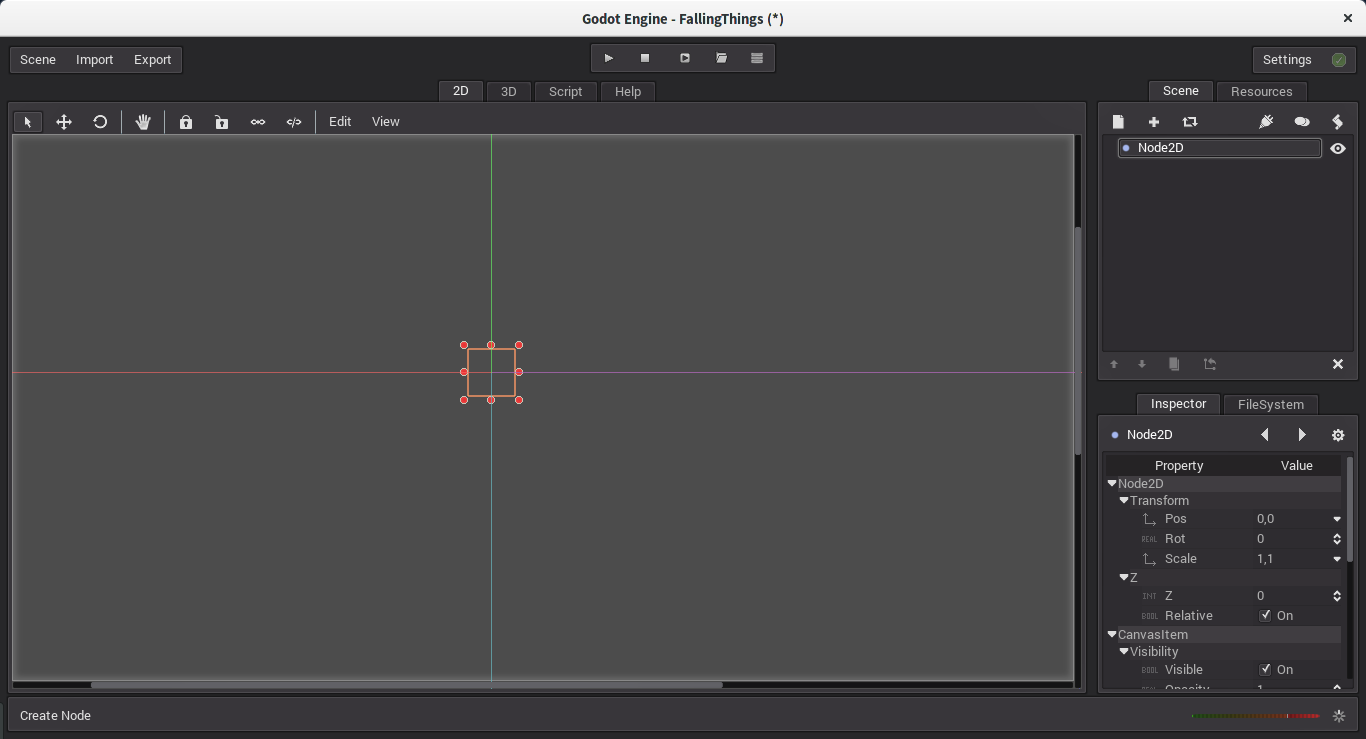
\includegraphics[width=12cm]{img/lvl1-screen7.png}
  \end{center}
  \caption{\label{lvl1-screen7} Notre tout premier noeud ! N'est-il pas joli ?}
\end{figure}

Votre écran devrait ressembler fortement à celui de la figure \ref{lvl1-screen7}. Godot a gentiment fait plusieurs choses :

\begin{itemize}
\item Fait passer la fenêtre en mode 2D, si ce n'était pas déjà fait.
\item Ajouté un objet \codeintext{Node2D} dans l'onglet \emph{Scene} en haut à droite.
\item Sélectionné le \emph{noeud} et affiché ses \emph{propriétés} dans l'\emph{inspecteur} en bas à droite.
\item Affiché un petit rectangle qui représente notre noeud sur l'écran.
\end{itemize}

Le petit rectangle permet de manipuler le \emph{noeud}, mais pour l'instant nous n'allons pas en avoir besoin, et pour être sûr de ne pas faire de bêtise, nous allons nous prémunir de nos propres actions en verrouillant le noeud. Pour ce faire, cherchez le bouton représentant un cadenas juste au dessus de la vue 2D du jeu, comme à la figure \ref{lvl1-lock}.

\begin{figure}
  \begin{center}
    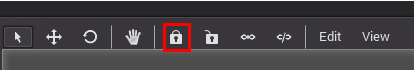
\includegraphics[width=5cm]{img/lvl1-lock.png}
  \end{center}
  \caption{\label{lvl1-lock} Ce petit cadenas peut vous sauver la vie !}
\end{figure}

Vous verrez un cadenas apparaître dans l'onglet \emph{Scene} ainsi que sur dans la vue 2D elle-même, et il signifie que vous ne pouvez pas modifier le \emph{noeud}. Cela parait un peu bizarre de vouloir restreindre ce qu'on peut modifier dans son propre projet, mais il vaut toujours mieux verrouiller ce que vous n'utilisez pas pour le moment. Tant qu'à faire, il vaut mieux éviter de perdre des heures de travail à cause d'un redimenssionnement inopiné qu'on n'avait pas remarqué, n'est-ce pas ?

La dernière chose que nous devons faire, c'est renommer le \emph{noeud}. En effet, sans prendre cette bonne habitude, vous risquez de finir avec une \emph{scène} remplie d'objets nommés \codeintext{Node2D}, et bonne chance pour savoir lequel correspond à quoi.

Pour changer le nom d'un \emph{noeud}, double-cliquez simplement sur son nom dans l'onglet \emph{Scene}, et entrez un nouveau nom. Conseil : choisissez un nom concis, de préférence sans espaces ou caractères spéciaux (un peu comme si vous nommiez une variable). Vous devrez souvent référencer ses noms dans votre code, donc évitez-vous des erreurs inutiles et faites dans la sobriété.

\begin{figure}
  \begin{center}
    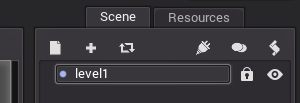
\includegraphics[width=4cm]{img/lvl1-rename.png}
  \end{center}
  \caption{\label{lvl1-rename} Probablement l'habitude la plus importante à attraper...}
\end{figure}

Une fois votre nom choisis, n'oubliez pas d'appuyer sur \emph{enter}, pour valider la saisie. De manière générale, Godot demande souvent de vous que vous validiez ce que vous venez d'entrer. Encore une bonne habitude... Si tout va bien, vous devriez avoir un \emph{noeud} renommé, comme à la figure \ref{lvl1-rename}.

Voilà, ouf, ça y est, notre premier noeud est en place. Que la longueur de cette section ne vous intimide pas : il a fallu aborder beaucoup de concepts en une fois, mais maintenant, l'ensemble pourra être condensé en une phrase à chaque nouveau \emph{noeud} qu'il faudra créer. N'est-ce pas merveilleux ?

En parlant de nouveaux \emph{noeuds}, que diriez-vous d'inclure un personnage à notre embryon de jeu ?

\section{Un peu de \emph{character} (accent british requis)}

Jusqu'ici, beaucoup de blabla pour finalement pas tellement de résultats, n'est-ce pas ? Accrochez vos ceintures, ça va changer !

\end{document}